\chapter{Airbus Ship Detection Challenge}
\lhead{Airbus Ship Detection Challenge}
\rhead{Radu-George Rusu}
\label{DatasetChapter}

This chapter presents the data set used for the experiment in this paper, the Kaggle competition that it was used in, and an analysis over how the data looks and can impact the experiments.

\begin{figure}[H]
	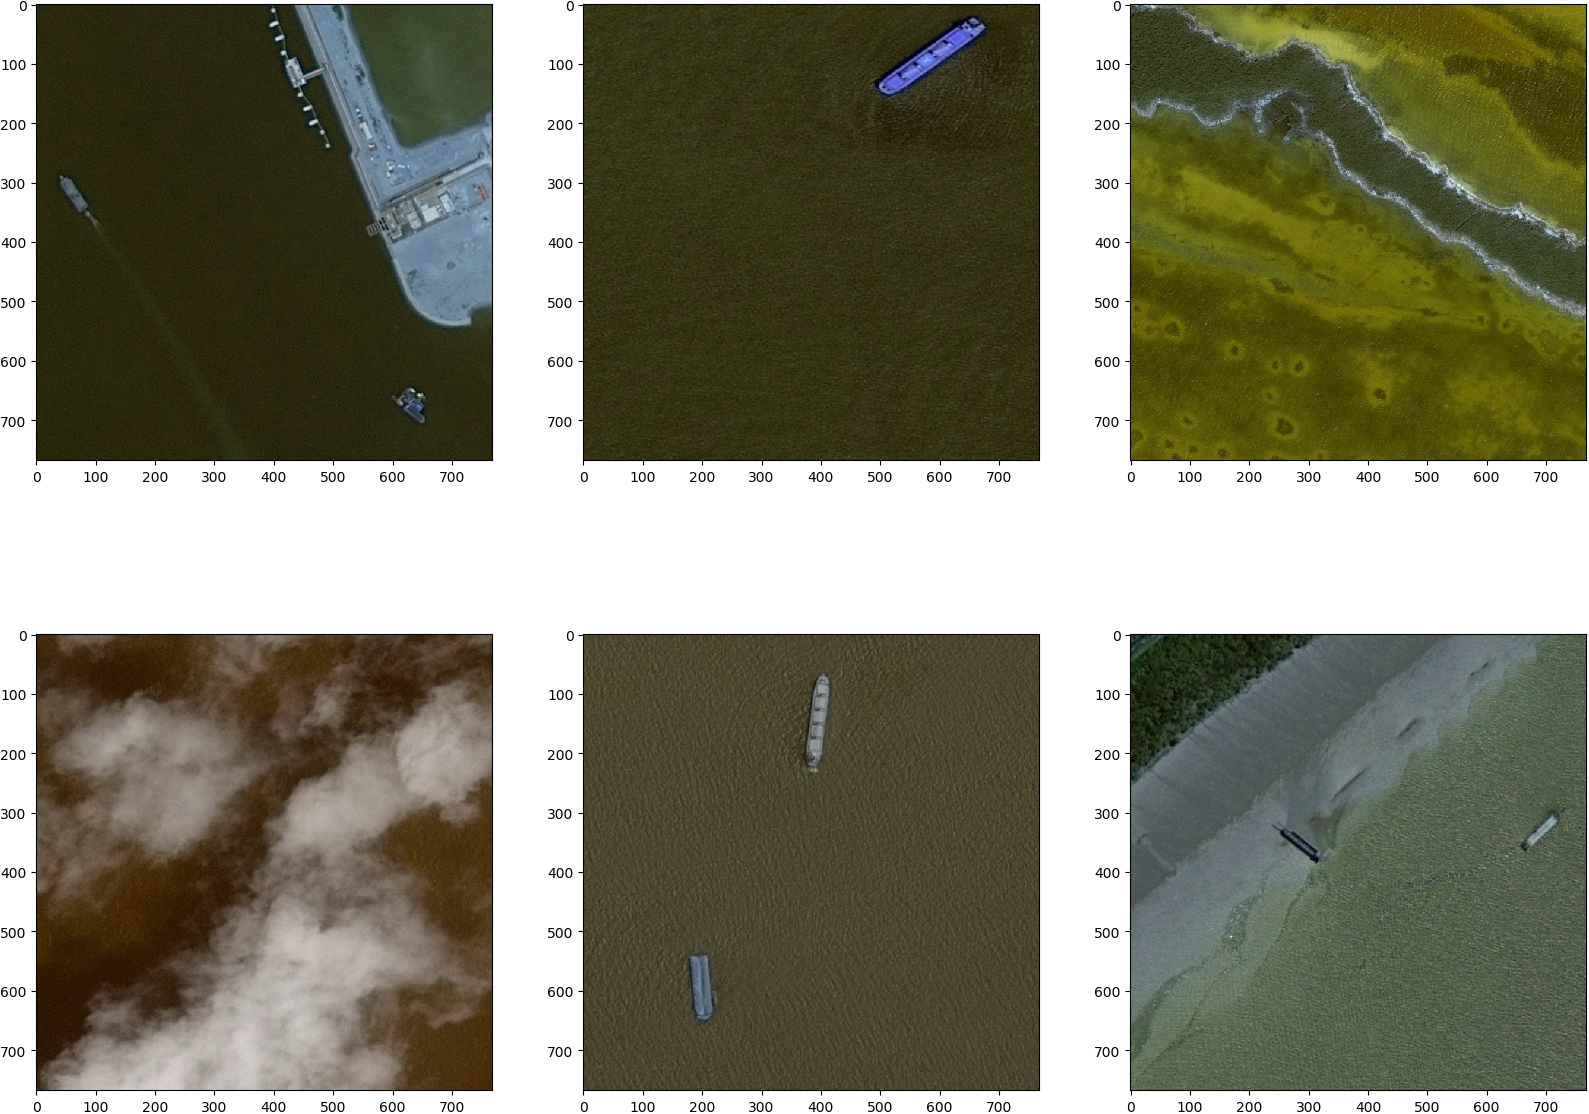
\includegraphics[width=\textwidth]{Pictures/003TrainingSetExamples.png}
	\caption{Training set examples}
	\label{TrainSetExample}
	%\textbf{Figure 2. Hill Climbing algorithm} [15]
\end{figure}

\section{Airbus Ship Dataset}
The Airbus Ship Dataset is an image dataset that was used in the Airbus Ship Detection Challenge \cite{AirbusDataSetChallenge} on \url{www.kaggle.com}. The aim of this competition is to detect ships inside an image taken from an aerial view. As the competition description says, this detection can help multiple organizations such as environmental organization and insurance companies to have knowledge of illegal activities done at sea. A few examples of the training set can be found in Figure \ref{TrainSetExample}.


\section{Analysis}
The competition provides both testing and training datasets in a large amount. The train set is composed of \textbf{231723} pictures, of size \textbf{768x768} pixels, in JPEG format, each of them having a set of pixels assigned as being ship pixels. To avoid specifying each pixel separately, for size reasons, the run length encoding is used. Every pixel is numbered from 1 to maximum size, top down, left right order. Pixel (1, 1) will have index 1, pixel (2, 1) index 2 etc. Run length encoding is formed of 2k numbers, the numbers in odd position (1 - indexed) specifies the starting index of a pixel ship sequence, and the ones in even position specifies the length of the sequence.
For example, the sequence: \textit{5 3 10 2}, encodes the ship pixels \textit{\{5, 6, 7, 10, 11\}}. Those encodings are provided via an \textbf{.csv} file, with two columns, \textbf{ImageId} and \textbf{EncodedPixels}. Also, in this file, every ship is given as a separate entry, so a picture can appear multiple times in this file and at least once. (See table \ref{traindfhead}). The figure \ref{OrigMask} shows the example images with their training masks.\\

\begin{table}[H]
	\centering
	\begin{tabular}{|c|c|l|}
		\hline
		ImageId & EncodedPixels \\ \hline
		00003e153.jpg & NaN         \\ \hline
		0001124c7.jpg & NaN         \\ \hline
		000155de5.jpg & 264661 17 265429 33 266197 33 266965 33 267733...         \\ \hline
		000194a2d.jpg & 360486 1 361252 4 362019 5 362785 8 363552 10 ...   \\ \hline
		000194a2d.jpg & 51834 9 52602 9 53370 9 54138 9 54906 9 55674 ...   \\ \hline
		000194a2d.jpg & 198320 10 199088 10 199856 10 200624 10 201392...  \\ \hline
		000194a2d.jpg & 55683 1 56451 1 57219 1 57987 1 58755 1 59523 ...  \\ \hline
		000194a2d.jpg & 254389 9 255157 17 255925 17 256693 17 257461 ...  \\ \hline
		0001b1832.jpg & NaN  \\ \hline
		00021ddc3.jpg & 108287 1 109054 3 109821 4 110588 5 111356 5 1...  \\ \hline
	\end{tabular}
	\captionof{table}{Train data set sample}\label{traindfhead}
\end{table}

The test set provided by the competition contains \textbf{15607} pictures of the same size as the ones in the training set, and the result that is submitted must also use the run length encoding described above.
\begin{figure}
	\centering
	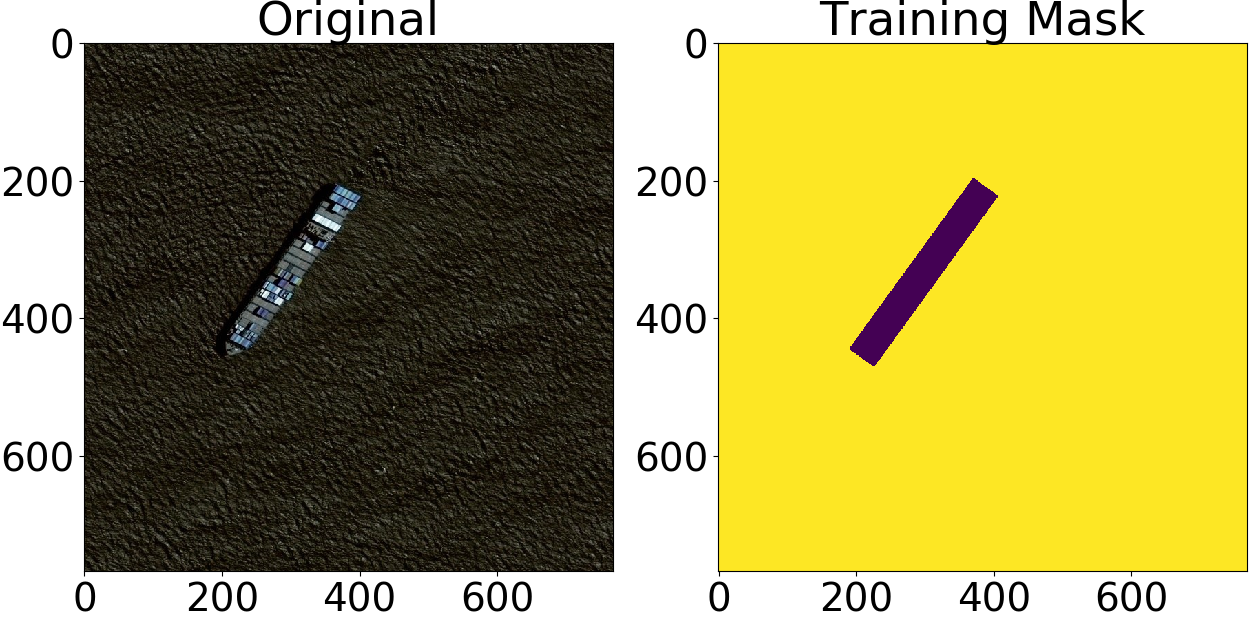
\includegraphics[width=0.75\textwidth]{Pictures/015OrigMaskExample1.png} \\
	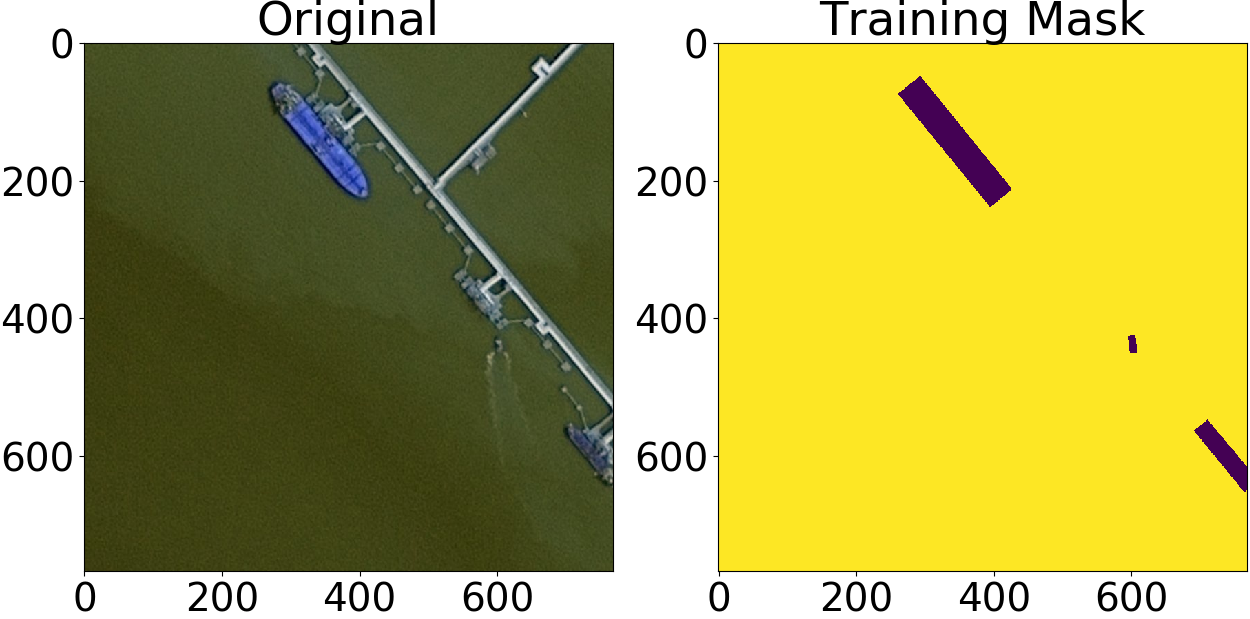
\includegraphics[width=0.75\textwidth]{Pictures/015OrigMaskExample2.png} \\
	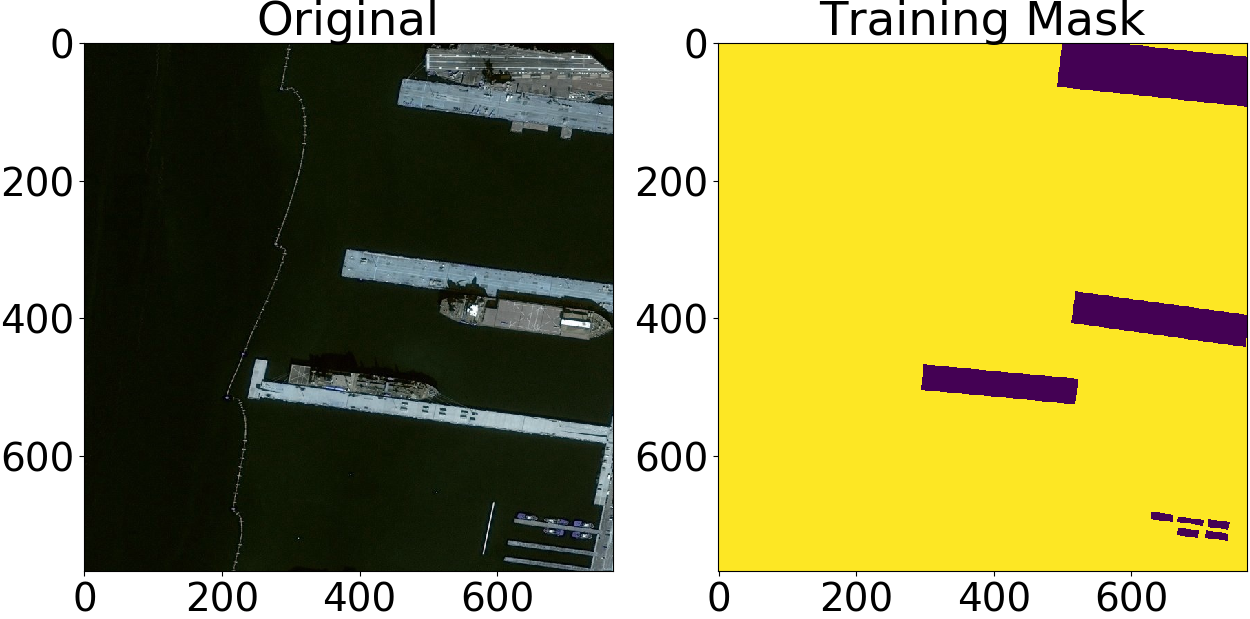
\includegraphics[width=0.75\textwidth]{Pictures/015OrigMaskExample3.png} 
	\caption{Original Images with Training Mask}
	\label{OrigMask}
\end{figure}

On a first inspection of this dataset, it can be observed that there are more pictures with no ship in them (0 encoded pixels), then the number of pictures with ships (as shown in table \ref{shipnoshiptable}). It can be seen that for every picture that has at least one ship in it, there are two pictures with no ship in it.

\begin{table}[H]
	\centering
	\begin{tabular}{|c|c|c|l|}
		\hline
		Total & No Ship Pictures & Ship Pictures \\ \hline
		231723 & 150000 & 81723 \\ \hline
	\end{tabular}
	\captionof{table}{Ship/no ship count training data}\label{shipnoshiptable}
\end{table}

Figure \ref{ShipNumberImage} has a histogram of number of images grouped by number of ships inside an image. The number of pictures that have only 1 ship stands out as being around 35\% from the total number of images with ship, and there are also pictures that contains up to 15 ships.

\begin{figure}
	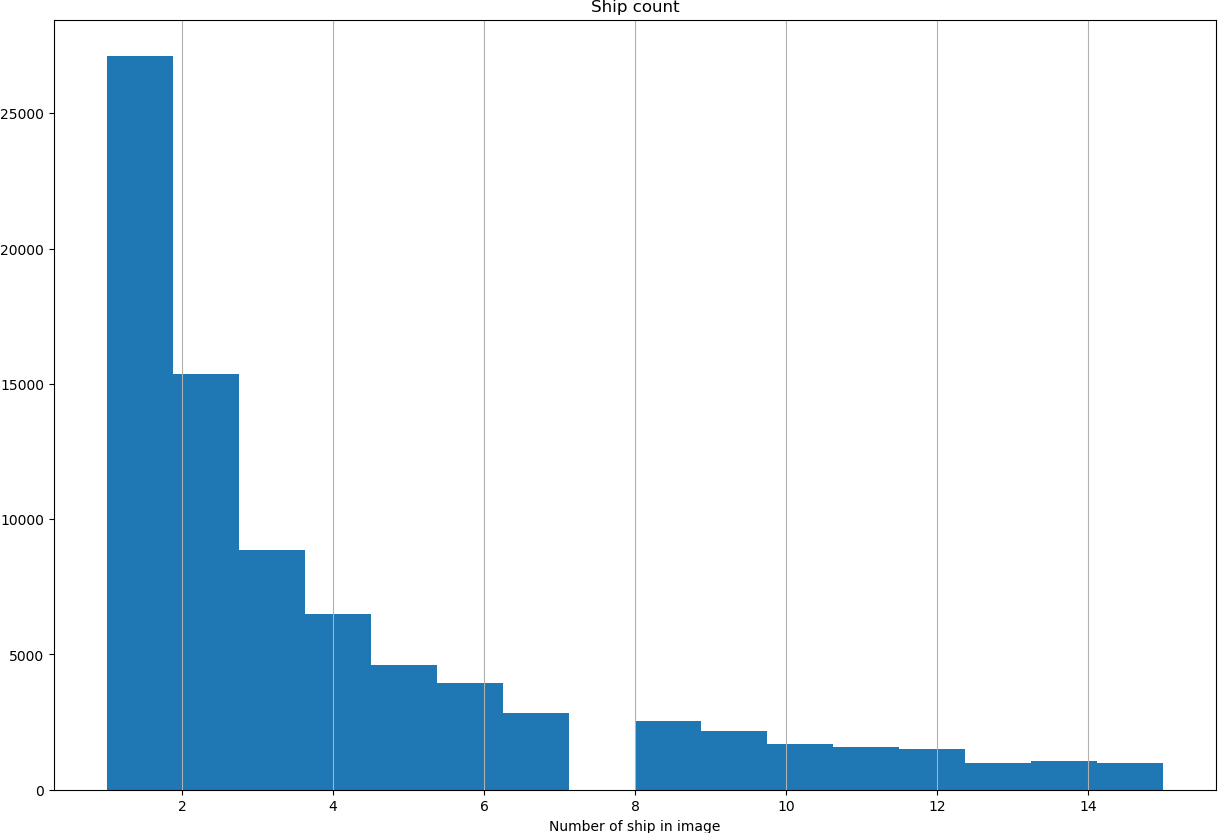
\includegraphics[width=\textwidth]{Pictures/001ShipNumberImage.png}
	\caption{ Number of ships/image}
	\label{ShipNumberImage}
	%\textbf{Figure 2. Hill Climbing algorithm} [15]
\end{figure}

The last metric that should be analyzed in this dataset is the ship size in pixels, to measure the magnitude of the task. As the table \ref{shipzisepixeltable} presents, the average size is around 1500 pixels, with half of the ships in the training set being under 408 pixels in size. Based on this, we can draw the conclusion that one ship that should be detected in the test set forms less than 0.0006\% of the entire image.

\begin{table}
	\centering
	\begin{tabular}{|c|c|c|c|c|c|l|}
		\hline
		Average & Min & Q1 & Median & Q3 & Max\\ \hline
		1,567.40 & 2.00	& 111 & 408.00 & 1550 & 25,904.00 \\ \hline
	\end{tabular}
	\captionof{table}{Ship size in pixels}\label{shipzisepixeltable}
\end{table}

\section{Evaluation Metric}
To evaluate possible solutions for this competition, the $F_2$ score was used. This is defined as follows:
\begin{itemize}
	\item We define a set of thresholds $T = \{0.5, 0.55, 0.6, \dots 0.95\}$.
	\item For every threshold $t \in T$:
	\item the $IoU$ between predicted pixels (pp) and true pixels (tp) of a ship is computed as $IoU = \frac{pp \cap pt}{pp \cup pt}$
	\item if this value is higher than $t$, then this item is consider a true positive (a hit)
	\item if this value is lower than $t$, then this is consider either a false negative (a predicted ship that has no true ship) or a false positive (there is no predicted ship for a true ship)
	\item the $F_2(t) =\frac{5TP(t)}{5TP(t) +4FN(t) + FP(t)}$ is computed
	\item the final score for an image is computed as $FS(image) = \frac{\sum_{t \in T} F_2(t)}{\big{|}T\big{|}}$
\end{itemize}

It is worth mentioning that this metric, in this form, penalizes more false negatives than false positives which means that it encourages rather not to predict a ship if the algorithm is not certain of the ship presence. This will have later implications in this paper. For this reason, the "no-machine algorithm" behaves really well, since this will give a percentage of images with no ships over a dataset.